\subsection{Phân tích phương sai một nhân tố (Single-factor ANOVA)}


Nhóm gọi:
\begin{itemize}
    \item Y: là một biến phụ thuộc (có tính liên tục).
\end{itemize}

- Nhóm gọi:
  + Y: là một biến phụ thuộc (có tính liên tục).
  + X: là một biến nhân tố hay biến giải thích (có tính phân loại).
- Yêu cầu đặt ra là đánh giá xem biến nhân tố X có ảnh hưởng đến biến phụ thuộc Y hay không?
- Giả thuyết:
  \[
  H_{0}: \mu_{1} = \mu_{2} = \mu_{3} = \dots = \mu_{n}
  \]
  \[
  H_{1}: \exists i, j \text{ sao cho } \mu_{i} \neq \mu_{j}
  \]

- Đọc dữ liệu từ file:
%   \begin{lstlisting}[language=R]
%   sxtk = read.csv("/Users/Windows10/Documents/Zalo Received Files/dirty_data.csv", header=T)
%   attach(sxtk)
%   \end{lstlisting}

- Bảng dữ liệu:
% \begin{lstlisting}[language=R]
% freq_table <- dt[,.N, by=coupon_discount]
% colnames(freq_table) <- c("coupon_discount", "count")
% \end{lstlisting}

\begin{figure}[!htbp]
    \centering
    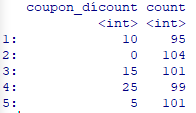
\includegraphics[width=0.4\linewidth]{graphics/5.3.1.png}
    \caption{Số lượng mặt hàng (count) theo từng loại chiết khấu (coupon\_discount)}
\end{figure}
